\section{Auswertung}
\label{sec:Auswertung}

Die Auswertung ist mithilfe von NumPy \cite{numpy}, Matplotlib \cite{matplotlib}, SciPy \cite{scipy} und Uncertainties \cite{uncertainties} erstellt.

\subsection{Horizontalfeldkomponente}

Nachdem der Tisch so ausgerichtet wurde, dass nur die Horizontalkomponente das Magnetfelds einen Beitrag leistet, wird die Transparenz minimiert und die Stromstärke für dieses Minimum gemessen.
Somit ergibt sich für die Horizontalfeldkomponente des Erdmagnetfeld mit Formel \ref{eq:B} ein Wert von 
\begin{equation*}
    B_\text{Erdmagnetfeld} = \SI{34.94}{\micro\tesla}.
\end{equation*}
Der Literaturwert für die Horizontalfeldkomponente des Erdmagnetfelds beträgt in Mitteleuropa ca. 
\begin{equation*}
    B_\text{Erdmagnetfeld} = \SI{20}{\micro\tesla}.
\end{equation*}

\subsection{Landé-Faktoren und Kernspins der Rubidium-Isotope} 
Im Folgenden steht der Index $\num{1}$ für $^{87}Rb$ und der Index $\num{2}$ für $^{85}Rb$. %richtig?

Die gemessenen Werte sind in Tabelle \ref{tab:all}
aufgelistet. Sie werden mit Formel \eqref{eq:B} in die jeweilige Magnetfeldstärke umgerechnet und die Magnetfeldstärken der Sweep- und der Horizontal-Spule werden für beide Peaks jeweils addiert.
\begin{table}\caption{Die Frequenz ist gegen den Strom der Sweep-Spule und den Strom der Horizontal-Spule für beide Peaks und die resultierenden $B$-Feldstärken aufgetragen.}
    \label{tab:all}
    \centering
    \sisetup{round-mode = places, round-integer-to-decimal=true}
     \begin{tabular}{S[round-precision=1] | S[round-precision=3] S[round-precision=3] S[round-precision=2] | S[round-precision=3] S[round-precision=3] S[round-precision=2]} 
        %\begin{tabular}{c | c c c  | c c c}  
    \toprule
{$f / \si{\kilo\hertz}$} & {$I_\text{sweep,1} / \si{\ampere}$} & {$I_\text{horizontal,1}/ \si{\ampere}$} & {$B_\text{1}/ \si{\micro\tesla}$} & {$I_\text{sweep,2}/ \si{\ampere}$} & {$I_\text{horizontal,2}/ \si{\ampere}$} & {$B_\text{1}/ \si{\micro\tesla}$} \\
\midrule
100     &   0.559   & 0.0       &  33.79 &   0.678 & 0.0         &  40.91  \\
200     &   0.424   & 0.0299    &  51.89 &   0.660 & 0.0299      &  66.13  \\
300     &   0.210   & 0.0599    &  65.29 &   0.567 & 0.0599      &  86.83  \\ 
400     &   0.281   & 0.0749    &  82.73 &   0.754 & 0.0749      &  111.27 \\
500     &   0.267   & 0.0899    &  95.03 &   0.858 & 0.0899      &  130.70 \\
600     &   0.239   & 0.107     &  109.13 &   0.949 & 0.107      &  151.98 \\  
700     &   0.233   & 0.125     &  124.55 &   0.704 & 0.149      &  174.02 \\  
800     &   0.316   & 0.137     &  140.09 &   0.685 & 0.174      &  193.93 \\  
900     &   0.337   & 0.149     &  151.88 &   0.587 & 0.209      &  219.58 \\  
1000    &   0.336   & 0.168     &  167.60 &   0.370 & 0.246      &  238.12 \\    

\bottomrule
\end{tabular}\end{table}
In Abb. \ref{fig:plot} werden die Magnetfeldstärken für beide Peaks gegen die Frequenz aufgetragen und eine Ausgleichsgerade wird jeweils durch die Messwerte gelegt. 
\begin{figure}
    \centering
    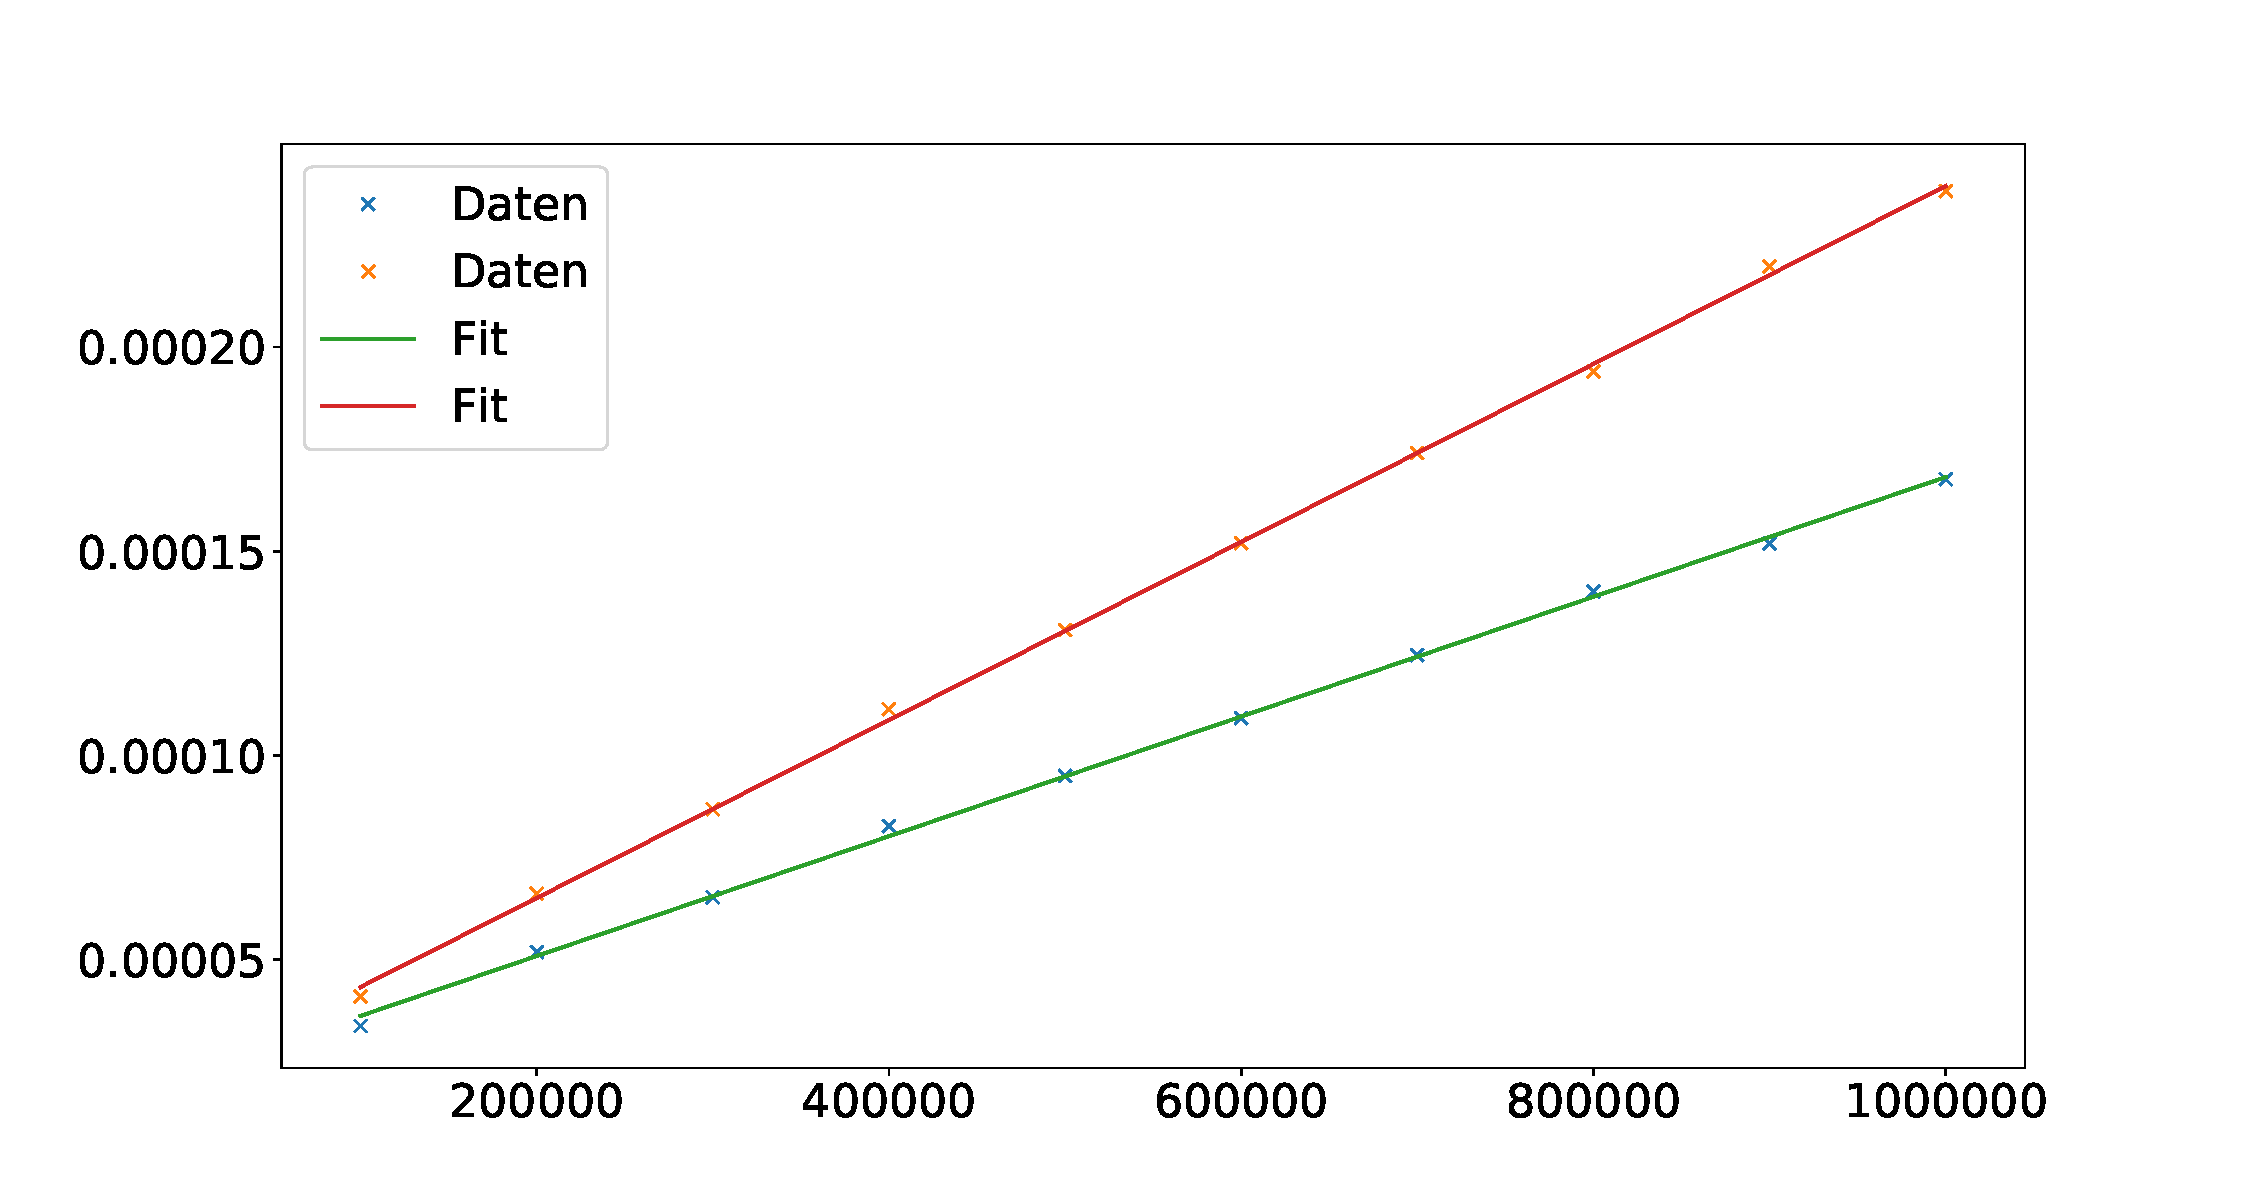
\includegraphics[width=0.9\textwidth]{plots/fits.pdf}
    \caption{Die Magnetfeldstärke $B$ beider Peaks ist gegen die Frequenz $f$ aufgetragen. Eine Ausgleichsgerade ist für beide Peaks durch die Werte gelegt worden, um daraus die Landé-Faktoren zu berechnen.}
    \label{fig:plot}
\end{figure}

Die Parameter der Ausgleichgeraden haben die folgenden Werte
\begin{align*}
    a_1 &= \SI{0.1465}{\micro\tesla\per\kilo\hertz} \\ %welche Einheit?
    a_2 &= \SI{0.2178}{\micro\tesla\per\kilo\hertz} \\
    b_1 &= \SI{21.6}{\micro\tesla} \\
    b_2 &= \SI{21.6}{\micro\tesla}
\end{align*}
Aus der Steigung lässt sich jeweils mit Formel \ref{eq:Zeeman} der Landé-Faktor bestimmen zu
\begin{align*}
    g_{\text{F},1} &= \num{488 \pm 6} \\
    g_{\text{F},2} &= \num{328 \pm 2.8}.
\end{align*}

Mit den Quantenzahlen $L = 0, S = \frac{1}{2}, J = \frac{1}{2}$ für Rubidium lässt sich Formel \ref{eq:I} nach $I$ umstellen zu
\begin{equation*}
    I = J (\frac{g_\text{J}}{g_\text{F}} -1).
\end{equation*} 
Aus den experimentell bestimmten Landé-Faktoren und dem Theoriewert $g_\text{J} = \num{2.0023}$, der aus Formel \ref{eq:gj} folgt, lässt sich der Kernspin für beide Peaks zu
\begin{align*}
    I_1 &= \num{1.553(23)} \\
    I_2 &= \num{2.552(26)}
\end{align*}
bestimmen. 
Die theoretischen Werte für die Kernspins sind
\begin{align*}
    I_1 &= \frac{3}{2} = \num{1.5} \\
    I_2 &= \frac{5}{2} = \num{2.5}.
\end{align*}


\subsection{Isotopenverhältnis}
Aus den beobachteten Amplituden bei $\SI{100}{\kilo\hertz}$, die in Abb. \ref{fig:Aufnahme} zu sehen sind, lässt sich das Isotopenverhältnis zwischen den beiden Isotopen $^{85}$Rb und $^{87}$Rb ablesen
\begin{equation*}
    \frac{440\text{px}}{216\text{px}} = \num{2.037}. 
\end{equation*}
\begin{figure}
    \centering
    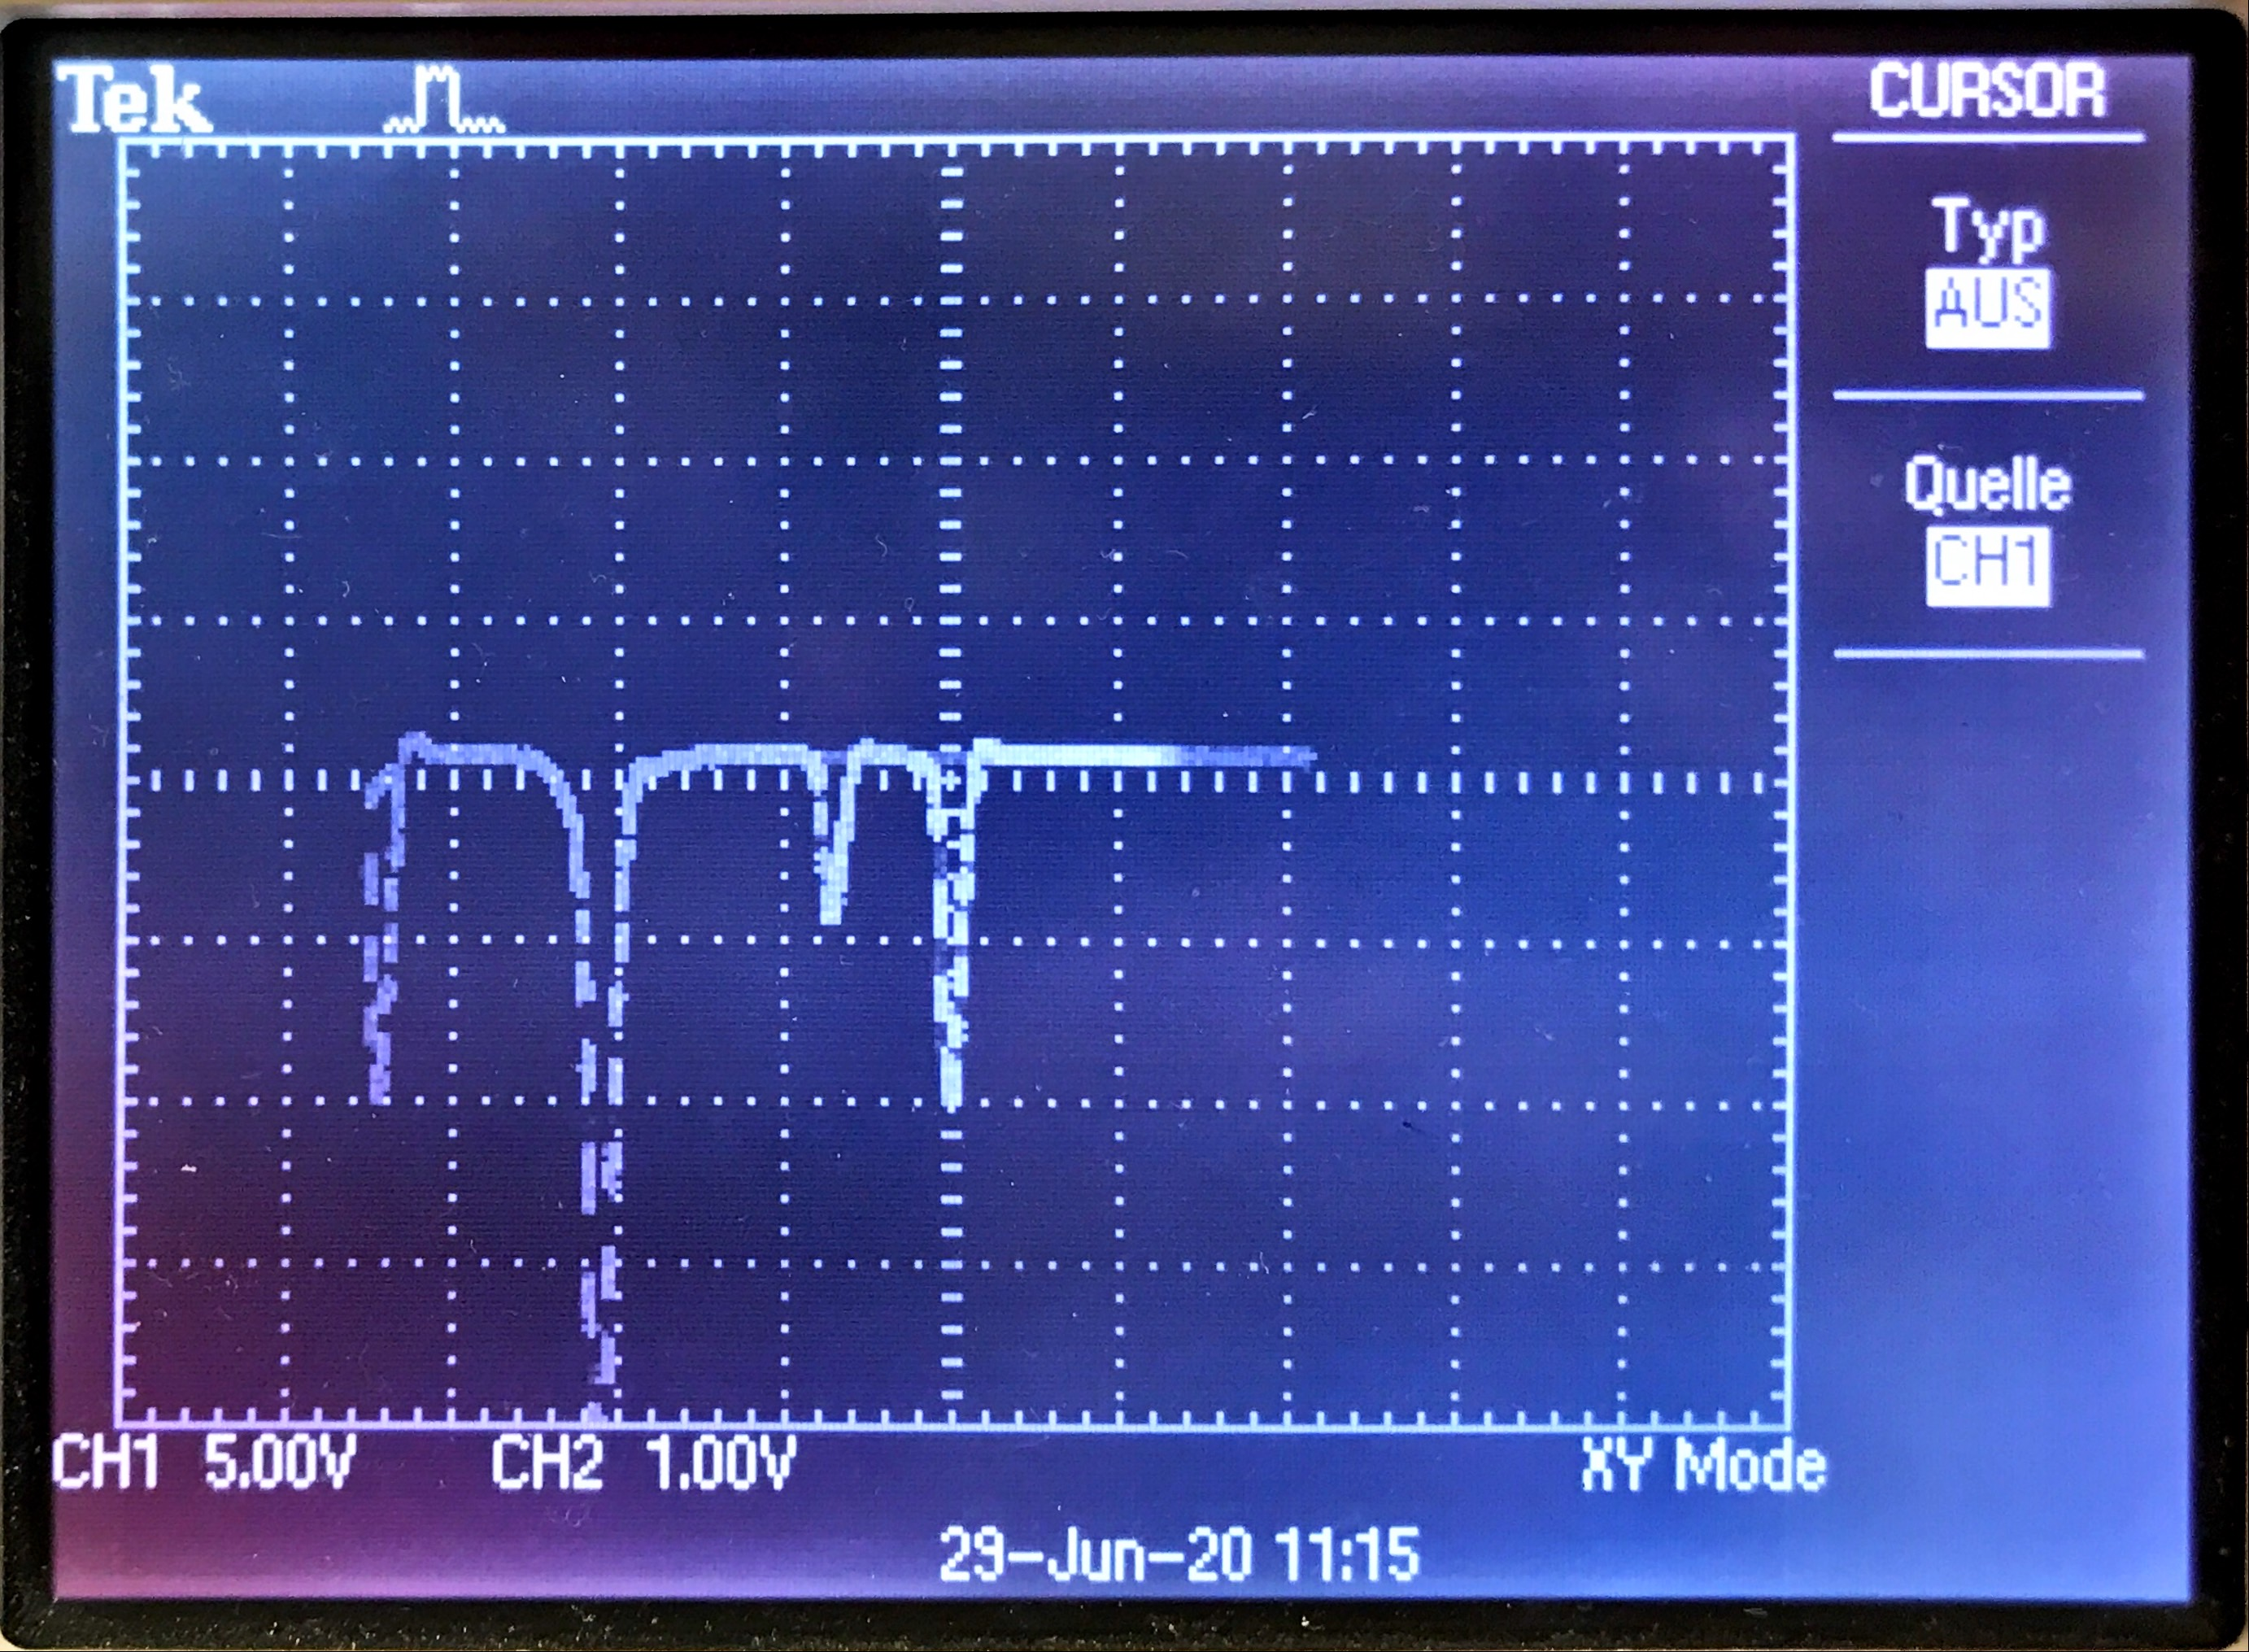
\includegraphics[width=0.8\textwidth]{fotos/Aufnahme.JPG}
    \caption{Eine typische Aufnahme bei $\SI{100}{\kilo\hertz}$ um das Verhältnis zwischen den beiden Isotopen $^{85}$Rb und $^{87}$Rb festzustellen.}
    \label{fig:Aufnahme}
\end{figure}
In der Natur beträgt das Verhältnis
\begin{equation*}
    \frac{\num{72.168}}{\num{27.835}} = \num{2.593}.
\end{equation*}
